%\usepackage{flafter}  % Don't place floats before their definition


\chapter{\label{chap:localExpansion}Local Expansion of Nonlocal Interactions}


I investigate the validity of expanding a nonlocal scalar potential $V(\vecrp,\vec{r})$ around a small nonlocality, i.e. when the potential is nearly diagonal in $|\vec{r}-\vecrp|$. 


\begin{section}{Expanding the Nonlocal Potential}
A two-body nonlocal potential takes the form $V(\vecrp,\vec{r})$ and the coordinate dependent part may be evaluated as
\begin{equation}\label{eq:nonlocaldef}
\braket{n' l' m'| V | n l m}=\int d^3r\:d^3r'\:R^*_{n',l'}(r') Y^*_{l',m'}(\hat{r}') V(\vecrp,\vec{r}) R_{n,l}(r) Y_{l,m}(\hat{r}).
\end{equation}
Throughout, we will assume that the potential is a scalar operator. Because nonlocal potentials require greater computational resources, it would be desirable to find a suitable local approximation. Intuitively, we can imagine that the potential $V(r,r')$ is nearly local. We take this to mean that it the contribution to the matrix element is small when $\vec{r}-\vecrp$ is large. We thus make a coordinate change with unit Jacobian to \eqref{eq:nonlocaldef}. A suitable choice of coordinates is the linear combination
\begin{equation}\label{eq:coords}
\vec{r}_1=\frac{\vec{r}+\vecrp}{2},\vec{r}_2=\vec{r}-\vecrp
\end{equation}
for which our nonlocality condition reduces to the requirement that the potential falls off rapidly in $r_2$. In the interest of generating clear, compact expressions we will also use the convenient definitions
\begin{align}
F(\vecrp)&=R^*_{n',l'}(r') Y^*_{l',m'}(\hatrp)\\
G(\vec{r})&=R_{n,l}(r) Y_{l,m}(\hat{r})
\end{align}
In these coordinates, the matrix elements become 
\begin{equation}
\bra{n' l' m'} V \ket{ n l m}= \int d^3r_1\:d^3r_2\:F\left( \vec{r}_1-\frac{\vec{r}_2}{2} \right) V\left(\vec{r}_1-\frac{\vec{r}_2}{2},\vec{r}_1+\frac{\vec{r}_2}{2}\right) 
G\left( \vec{r}_1+\frac{\vec{r}_2}{2}\right).
\end{equation}
We then make a Taylor expansion of the wave functions $F$ and $G$ in the coordinate $\vec{r}_2$\footnote{For now, we do not expand the potential itself. Such an expansion can be helpful in evaluating the angular integrals for some of the density-dependent two-body terms of the previous chapter. This will be discussed in Section~\ref{sec:localChiral}.}. The three dimensional Taylor expansion can be written in Cartesian form as
\begin{align}\label{eq:TaylorExpansion}
F\left(\vec{r}_1-\frac{\vec{r}_2}{2}\right)&=F(\vec{r}_1)-\frac{1}{2}\vec{r}_2\cdot\vec{\nabla}_1 F(\vec{r}_1)+\frac{1}{2}\left(\frac{1}{2}\vec{r}_2\cdot\vec{\nabla}_1\right)\left(\frac{1}{2}\vec{r}_2\cdot\vec{\nabla}_1\right)F(\vec{r}_1)+\dots 
\\
G\left(\vec{r}_1+\frac{\vec{r}_2}{2}\right)&=G(\vec{r}_1)+\frac{1}{2}\vec{r}_2\cdot\vec{\nabla}_1 G(\vec{r}_1)+\frac{1}{2}\left(\frac{1}{2}\vec{r}_2\cdot\vec{\nabla}_1\right)\left(\frac{1}{2}\vec{r}_2\cdot\vec{\nabla}_1\right)G(\vec{r}_1)+\dots
\end{align}
Note that the asymmetric choice of coordinates made in \eqref{eq:coords} has the desirable effect of allowing one to expand the wave functions around $\vec{r}_1$ without any additional constants. Compare this expansion also with that of \cite{0954-3899-26-3-310}, where only the function $G(\vec{r})$ is expanded around $\vec{r}=\vecrp$. Plugging this expansion in up to second order 
\begin{equation}\label{eq:expansionCartesian}
\begin{split}
\braket{n' l' m'| V | n l m} &= \int d^3r_1\: F(\vec{r}_1)\left[\int d^3r_2\:\left\{V\left(\vec{r}_1-\frac{\vec{r}_2}{2},\vec{r}_1+\frac{\vec{r}_2}{2}\right) \right.\right. \\
&-\frac{1}{2} \left(\lvec{\nabla}_1\cdot\vec{r}_2\: V\left(\vec{r}_1-\frac{\vec{r}_2}{2},\vec{r}_1+\frac{\vec{r}_2}{2}\right) -
V\left(\vec{r}_1-\frac{\vec{r}_2}{2},\vec{r}_1+\frac{\vec{r}_2}{2}\right) \vec{r}_2\cdot\vec{\nabla}_1
\right)\\
&-\frac{1}{4}\lvec{\nabla}_1\cdot\vec{r}_2\: V\left(\vec{r}_1-\frac{\vec{r}_2}{2},\vec{r}_1+\frac{\vec{r}_2}{2}\right) \vec{r}_2\cdot\vec{\nabla}_1\\
&+\frac{1}{8}\left(\lvec{\nabla}_{1}\cdot\vec{r}_2\right)^2 V\left(\vec{r}_1-\frac{\vec{r}_2}{2},\vec{r}_1+\frac{\vec{r}_2}{2}\right) 
\left.\left.+\frac{1}{8} V\left(\vec{r}_1-\frac{\vec{r}_2}{2},\vec{r}_1+\frac{\vec{r}_2}{2}\right) \left(\vec{r}_2\cdot\vec{\nabla}_{1}\right)^2+\dots \right\}\right]G(\vec{r}_1)
\end{split}
\end{equation}

Alternately, we can also express the expansion \eqref{eq:TaylorExpansion} in terms of spherical tensor operators,
\begin{align}
\begin{split}
F\left(\vec{r}_1-\frac{\vec{r}_2}{2}\right)=
F(\vec{r}_1)&-\frac{1}{2}\sqrt{\frac{4\pi}{3}}\sum_{m}(-1)^m r_2 Y_{1,m}(\hat{r}_2) \vec{\nabla}_{1,-m} F(\vec{r}_1) \\
&\hspace{.5cm}+\frac{1}{8}\frac{4\pi}{3}\sum_{m,m'}(-1)^{m+m'}r_2^2 Y_{1,m}(\hat{r}_2)Y_{1,m'}(\hat{r}_2)\vec{\nabla}_{1,-m}\vec{\nabla}_{1,-m'}F(\vec{r}_1)
+\dots 
\end{split}
\end{align}
Inserting this expansion of the wave functions, the matrix elements \eqref{eq:nonlocaldef} are given by,
\begin{equation}\label{eq:expansionSpherical}
\begin{split}
\braket{n' l' m'| V | n l m} &= \int d^3r_1\: F(\vec{r}_1)\left[\int d^3r_2\:\left\{V\left(\vec{r}_1-\frac{\vec{r}_2}{2},\vec{r}_1+\frac{\vec{r}_2}{2}\right) \right.\right. \\
&-\frac{1}{2}\sqrt{\frac{4\pi}{3}}\sum_m (-1)^m \lvec{\nabla}_{1,-m} r_2Y_{1,m}(\hat{r}_2)V\left(\vec{r}_1-\frac{\vec{r}_2}{2},\vec{r}_1+\frac{\vec{r}_2}{2}\right)\\
&+\frac{1}{2}\sqrt{\frac{4\pi}{3}}\sum_m (-1)^m r_2Y_{1,m}(\hat{r}_2)V\left(\vec{r}_1-\frac{\vec{r}_2}{2},\vec{r}_1+\frac{\vec{r}_2}{2}\right) \vec{\nabla}_{1,-m} \\
&-\frac{1}{4}\frac{4\pi}{3}\sum_{m,m'}(-1)^{m+m'}\lvec{\nabla}_{1,-m} r_2^2 Y_{1,m}(\hat{r}_2)Y_{1,m'}(\hat{r}_2)V\left(\vec{r}_1-\frac{\vec{r}_2}{2},\vec{r}_1+\frac{\vec{r}_2}{2}\right) \vec{\nabla}_{1,-m'}\\
&+\frac{1}{8}\frac{4\pi}{3}\sum_{m,m'}(-1)^{m+m'}\lvec{\nabla}_{1,-m}\lvec{\nabla}_{1,-m'} r_2^2 Y_{1,m}(\hat{r}_2)Y_{1,m'}(\hat{r}_2)V\left(\vec{r}_1-\frac{\vec{r}_2}{2},\vec{r}_1+\frac{\vec{r}_2}{2}\right) \\
&\left.\left.+\frac{1}{8}\frac{4\pi}{3}\sum_{m,m'}(-1)^{m+m'} r_2^2 Y_{1,m}(\hat{r}_2)Y_{1,m'}(\hat{r}_2)V\left(\vec{r}_1-\frac{\vec{r}_2}{2},\vec{r}_1+\frac{\vec{r}_2}{2}\right)\vec{\nabla}_{1,-m}\vec{\nabla}_{1,-m'}+\dots \right\}\right]G(\vec{r}_1)
\end{split}
\end{equation}

Eliminating the dependence on either $\vec{r}_1$ or $\vec{r}_2$ makes an effective local approximation to the original matrix elements. In the following sections, we discuss approaches to evaluate the $\vec{r}_2$ integral for a toy potential (Section~\ref{sec:toyModel}) and three different types of terms from the two-body effective potential (Section~\ref{sec:localChiral}).

\end{section}

%%%%%%%%%%%%%%%%%%%%%%%%%%%%%%%%%%%%%%%%%%%%%%%%
\begin{section}{Exploration Using Model Potentials\label{sec:toyModel}}

In order to explore the convergence of the local Taylor approximation, we evaluate the matrix elements of simple potentials in a harmonic oscillator basis and compare them with the full nonlocal matrix elements.  We expect the convergence to be best for potentials which are nearly diagonal in $|\vec{r}-\vecrp|$. To test this hypothesis, we will consider two simple toy potentials. In particular, we want the function $g(|\vec{r}-\vecrp|)$ to have a tunable parameter controlling the nonlocality, with a local potential in some limit. As an example, consider the Gaussian potential
\begin{equation}\label{eq:gaussToy}
V(\vec{r},\vecrp)=\left(\frac{2}{\pi\lambda_1^2}\right)^{3/2}e^{-(\vec{r}+\vecrp)^2/2\lambda_1^2} \left(\frac{1}{2\pi\lambda_2^2}\right)^{3/2}e^{-(\vec{r}-\vecrp)^2/2\lambda_2^2}.
\end{equation}
We can see that in the limit $\lambda_2\rightarrow 0$ the potential becomes local, i.e.
\begin{equation}
\lim_{\lambda_2\rightarrow0}V(\vec{r},\vecrp)=\left(\frac{2}{\pi\lambda_1^2}\right)^{3/2}e^{-(\vec{r}+\vecrp)^2/2\lambda_1^2}\delta^{(3)}(\vec{r}-\vecrp).
\end{equation}

Another simple potential of this form is
\begin{equation}
V(\vec{r},\vecrp)=\frac{e^{-|\vec{r}+\vecrp|/\lambda_1}}{\pi\lambda_1^3}\frac{e^{-|\vec{r}-\vecrp|/\lambda_2}}{8\pi\lambda_2^3}.
\end{equation}

A potential which can be factored as 
\begin{equation}
V(\vecrp,\vec{r})=f(|\vec{r}+\vecrp|)g(|\vec{r}-\vecrp|)
\end{equation}
for some scalar functions $f$ and $g$ is particularly easy to evaluate in the form \eqref{eq:expansionSpherical}. Any operator of this form is guaranteed to be Hermitian, as the magnitudes $|\vec{r}+\vecrp|$ and $|\vec{r}-\vecrp|$ are necessarily invariant under exchanging $\vec{r} \leftrightarrow \vecrp$. There are three different combinations of spherical harmonics and the nonlocal potential to consider when evaluating the $\vec{r}_2$ integral to second order. First is the average of the potential over $\vec{r}_2$ which I will denote as $V^1(\vec{r}_1)$:
\begin{equation}\label{eq:V0}
\begin{split}
V^0(\vec{r}_1)=&\int d^3r_2\: V\left(\vec{r}_1-\frac{\vec{r}_2}{2},\vec{r}_1+\frac{\vec{r}_2}{2}\right) \\
=&\hspace{.1cm}4\pi f(2r_1) \int dr_2\: r_2^2 g(r_2)
\end{split}
\end{equation}
The first order contributions vanish for a potential of this form due to the angular integration over a single spherical harmonic,
\begin{equation}\label{eq:V1}
V^1(\vec{r}_1)=\int d^3r_2\:  r_2Y_{1,m}(\hat{r}_2)V\left(\vec{r}_1-\frac{\vec{r}_2}{2},\vec{r}_1+\frac{\vec{r}_2}{2}\right)=0.
\end{equation}
The second order terms all have the same $r_2$ dependence, but depend on $m$ and $m'$. I will denote these as $V^2_{m,m'}(\vec{r}_1)$. They are given by,
\begin{equation}\begin{split}
\label{eq:V2}
V^2_{m,m'}(\vec{r}_1)&=\int d^3r_2\: r_2^2Y_{1,m}(\hat{r}_2)Y_{1,m'}(\hat{r}_2)V\left(\vec{r}_1-\frac{\vec{r}_2}{2},\vec{r}_1+\frac{\vec{r}_2}{2}\right) \\
&=(-1)^{m'}\int d^3r_2\: r_2^2Y_{1,m}(\hat{r}_2)Y^*_{1,-m'}(\hat{r}_2)V\left(\vec{r}_1-\frac{\vec{r}_2}{2},\vec{r}_1+\frac{\vec{r}_2}{2}\right)\\
&=(-1)^m\delta_{m,-m'}\int d r_2 \:r_2^4 V\left(\vec{r}_1-\frac{\vec{r}_2}{2},\vec{r}_1+\frac{\vec{r}_2}{2}\right).
\end{split}
\end{equation}
For further simplicity, we can rewrite $V^2_{m,m'}(\vec{r}_1)=\delta_{m,-m'}V^2(\vec{r}_1)$.

With these definitions, we can rewrite \eqref{eq:expansionSpherical} more compactly as,
\begin{equation}\label{eq:expansion2}
\begin{split}
\braket{n' l' m'| V | n l m} =  \int d^3r\: F(\vec{r})\left( \vphantom{\frac{1}{2}}V_1(\vec{r})\right.&-\frac{1}{4}\frac{4\pi}{3}\sum_m(-1)^m \lvec{\nabla}_{m}  V_2(\vec{r}) \vec{\nabla}_{-m} \\
&\left.+\frac{1}{8}\frac{4\pi}{3}\lvec{\nabla}\cdot\lvec{\nabla} V_2(\vec{r})+\frac{1}{8}\frac{4\pi}{3}V_2(\vec{r})\vec{\nabla}\cdot\vec{\nabla}+\dots\right) G(\vec{r}_1).
\end{split}
\end{equation}
Note that the integrals in \cref{eq:V0,eq:V1,eq:V2}  are equivalent to calculating moments of the potential with respect to $\vec{r}_2$. These matrix elements may be evaluated in a harmonic oscillator basis using the formulas presented in Appendix~\ref{app:HObasis}.

Evaluating the full nonlocal matrix elements requires a six-dimensional integration (including oscillatory behavior when the matrix elements are taken between states with $l$ nonzero). Monte Carlo (MC) integration strategies are considered state of the art for high-dimensional integration. I have evaluated the matrix elements using the {\ttfamily{Cuba}} library~\cite{Hahn200578}. The importance sampling strategies in the four MC integration techniques lead to convergence more reliably and with fewer samples than Mathematica's native implementations for the integrals at hand. In the following figures I used the {\ttfamily Vegas} algorithm.

\begin{figure}[htb]
\centering 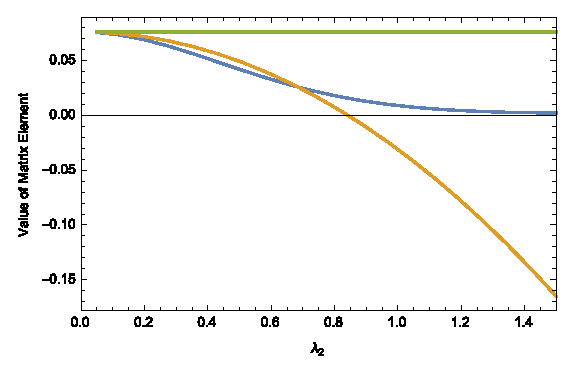
\includegraphics[width=0.6\textwidth]{LocalExpansion/Figures/ToyPotential000000} 
\caption[Matrix elements of the toy potential with varying $\lambda_2$]{Matrix elements of $\braket{n'=0,\: l'=0,\: m_l'=0 |\, V/\hbar\omega \, | n=0,\: l=0,\: m_l=0}$ for $r=b=\lambda_1$ as a function of $\lambda_2/b$. The blue line shows the exact numerically evaluated matrix elements, while the orange line shows the second order Taylor approximation. As expected, the second order local approximation is very good when the non-locality measure $\lambda_2/b$ is small.
\label{fig:gaussToy1}}
\end{figure}

Matrix elements of the potential \eqref{eq:gaussToy} compare qualitatively as expected. First, we see that the exact values and the Taylor approximation converge for $\lambda_2\rightarrow 0$ in \Cref{fig:gaussToy1} but that the error increases as the range parameter $\lambda_2/b$ becomes non-perturbatively large. \Cref{fig:gaussToy2} demonstrates that the convergence is essentially independent of $\lambda_1$. 

%One interesting observation in the second order approximation is that the second derivative in $\lambda_2$ of the matrix elements is strictly negative for all of the channels tested, although this is not true for the exact results. Does the addition of fourth order terms (the third order terms are zero) introduce contributions which change this situation?

\begin{figure}[htb]
\centering 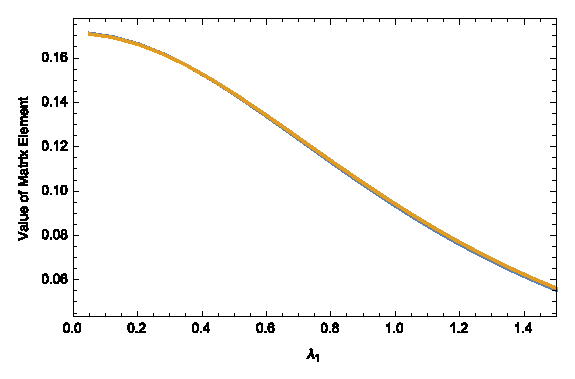
\includegraphics[width=0.6\textwidth]{LocalExpansion/Figures/ToyPotential000000l1} 
\caption[Matrix elements of the toy potential with varying $\lambda_1$]{Matrix elements of $\braket{n'=0,\: l'=0,\: m_l'=0 |\, V/\hbar\omega \,| n=0,\: l=0,\: m_l=0}$ for $r/b=1$, $\lambda_2/b=0.05$ as a function of $\lambda_1/b$. The blue line shows the exact numerically evaluated matrix elements, while the orange line shows the second order Taylor approximation. This plot demonstrates that the strength of the local term does not effect the convergence.
\label{fig:gaussToy2}}
\end{figure}

\end{section}

\begin{section}{Second Order Local Expansion of the Two-Body Effective Chiral Potential\label{sec:localChiral}}

In this section we consider the problem of finding the second order expansion of the density-dependent two-body effective potential. The easiest term in the density-dependent two-body effective potential to expand is $\veff^D$, due to the delta functions $\w{0}{0}{0}{\rot}$. We apply the spherical tensor form of the expansion \eqref{eq:expansionSpherical} and integrate over $\vec{r}_2$ using the delta function to obtain

\begin{align}
&\hspace{-.4cm}V^{1PE,\text{Nonlocal}}_{12,\text{eff}}= \frac{-c_D g_A}{8F_\pi^4 \Lambda_\chi}\frac{m_\pi^6}{4\pi} \left\{\phantom{\frac{-c_D g_Am_\pi^6}{8 F_\pi^4 \Lambda_\chi}}\right.\\
&\left[\left(\lvec{\nabla}^2r_{12}^2+\frac{8\pi}{15}\left[\lvec{\nabla}\otimes \lvec{\nabla}\right]_2\cdot \vec{Y}_2(\Omega_{12})r_{12}^2 \right) \rhohat{0}{2 r_{12}}\left(\taudot W^{\text{LR}}_{1PE}(2\rot)+3\w{0}{1}{0}{r_{12}} \right)\right. \\
%
&\hspace{.7cm}+\lvec{\nabla}\cdot\vec{r}_{12} \,\rhohat{0}{2 r_{12}} \left(\taudot W^{\text{LR}}_{1PE}(2\rot)+3\w{0}{1}{0}{r_{12}} \right)\vec{r}_{12}\cdot\vec{\nabla} \\
%
&\hspace{.7cm}+\left.\rhohat{0}{2 r_{12}} \left(\taudot W^{\text{LR}}_{1PE}(2\rot)+3\w{0}{1}{0}{r_{12}} \right)\left(r_{12}^2 \vec{\nabla}^2+\frac{8\pi}{15}r_{12}^2\vec{Y}_2(\Omega_{12})\cdot\left[\vec{\nabla}\otimes \vec{\nabla}\right]_2 \right)\right] \\
%
%
+&\left[\left(\lvec{\nabla}^2r_{12}^2+\frac{8\pi}{15}\left[\lvec{\nabla}\otimes \lvec{\nabla}\right]_2\cdot \vec{Y}_2(\Omega_{12})r_{12}^2 \right) \rhohat{1}{2 r_{12}} \left(\taudot W^{\text{LR}}_{1PE}(2\rot)-\w{0}{1}{0}{r_{12}} \right)\right. \\
%
&\hspace{.7cm}+\lvec{\nabla}\cdot\vec{r}_{12}\, \rhohat{1}{2 r_{12}} \left(\taudot W^{\text{LR}}_{1PE}(2\rot)-\w{0}{1}{0}{r_{12}} \right)\vec{r}_{12}\cdot\vec{\nabla} \\
%
&\left.\hspace{.7cm}+\left.\rhohat{1}{2 r_{12}}\left(\taudot W^{\text{LR}}_{1PE}(2\rot)-\w{0}{1}{0}{r_{12}} \right)\left(r_{12}^2 \vec{\nabla}^2+\frac{8\pi}{15}r_{12}^2\vec{Y}_2(\Omega_{12})\cdot\left[\vec{\nabla}\otimes \vec{\nabla}\right]_2 \right)\right]\right\}.
\end{align}
To make the notation consistent with standard two-body potentials, the coordinate $\vec{r}_1$ has been renamed to $\vec{r}_{12}$ after performing the integration. It should be interpreted as the usual relative Jacobi coordinate of the two particle system and the potential is now fully local.

Unfortunately, the remaining terms are more difficult to integrate. We show here how the scalar functions in the expressions from Section~\ref{sec:coord} remain dependent on the magnitudes of linear combinations of coordinates and therefore complicate the angular integrals. A majority of the remaining nonlocal terms seen in Section~\ref{sec:coord} are of the form
%
\begin{equation}
V(\rot,\rotp)=f(r_{12})g(|\rot-\rotp |) \left[Y_{l}(\hat{r})\otimes Y_{l'}\left(\frac{\rot-\rotp}{|\rot-\rotp |}\right)\right]_{L M}\pm \rot\leftrightarrow \rotp.
\end{equation}
%
After substituting the new variables \eqref{eq:nonlocaldef}, we have
%
\begin{equation}\label{eq:r1r2Form1}
V(\vec{r}_1,\vec{r}_2)=f(|\vec{r}_1+\vec{r}_2/2|)g(r_2) \left[Y_{l}\left(\frac{\vec{r}_1+\vec{r}_2/2}{|\vec{r}_1+\vec{r}_2/2|}\right)\otimes Y_{l'}\left(\hat{r}_2\right)\right]_{L M} \pm \vec{r}_2\rightarrow -\vec{r}_2
\end{equation} 
%
We can rewrite the second spherical harmonic using a formula from \cite{varshalovich1988},
%
\begin{multline}
Y_{l'm'}\left(\frac{\rot-\rotp}{|\rot-\rotp |}\right) = \sum_{l=0}^{l'}(-1)^{l'+l}\sqrt{\frac{4\pi(2l+1)(2l'-2l+1)}{2l'+1}} \\
\times \rotpr^{l'-l} r_{12}^l |\rot-\rotp|^{-l'}\left[Y_{l}(\hat{r}_{12})\otimes Y_{l'-l}(\rotphat))\right]_{l'm'}
\end{multline}
With this substitution, \eqref{eq:r1r2Form1} becomes
\begin{multline}
V(\vec{r}_1,\vec{r}_2)=f(|\vec{r}_1+\vec{r}_2/2|)g(r_2) \\
\sum_{l''=0}^{l} \sqrt{\frac{4\pi(2l''+1)(2l-2l''+1)}{2l+1}} \;r_1^{l''} \left(\frac{r_2}{2}\right)^{l-l''}|\vec{r}_1+\vec{r}_2/2|^{-l} \\
 \Big[\big[Y_{l''}(\hat{r}_1) \otimes Y_{l-l''}(\hat{r}_2) \big]_l \otimes Y_{l'}\left(\hat{r}_2\right)\Big]_{L M} \pm \vec{r}_2 \rightarrow -\vec{r}_2
\end{multline}
Next, we can use the Wigner 6-$j$ symbol to recouple the three spherical harmonics, 
\begin{multline}
V(\vec{r}_1,\vec{r}_2)=f(|\vec{r}_1+\vec{r}_2/2|)g(r_2) 
\sum_{l''=0}^{l} \sqrt{4\pi(2l''+1)(2l-2l''+1)} \;r_1^{l''} \left(\frac{r_2}{2}\right)^{l-l''}|\vec{r}_1+\vec{r}_2/2|^{-l} \\
\sum_{l'''} (-1)^{l+l'+L} \sqrt{(2l'''+1)} \sixj{l''}{l-l''}{l}{l'}{L}{l'''} \Big[\big[Y_{l'}(\hat{r}_2) \otimes Y_{l-l''}(\hat{r}_2) \big]_{l'''} \otimes Y_{l''}\left(\hat{r}_1\right)\Big]_{L M} \\
\pm \vec{r}_2 \rightarrow -\vec{r}_2
\end{multline}
where the sum over $l'''$ includes all values for which the 6-$j$ symbol is nonzero. Finally we combine the coupled $r_2$ spherical harmonics\footnote{$\sqrt{4\pi(2l+1)}[Y_{l_1}(\hat{r})\otimes Y_{l_2}(\hat{r})]_{lm}=\sqrt{(2l_1+1)(2l_2+1)}\braket{l_1\,0,l_2\,0|l_1\,l_2\,l\,0}Y_{lm}(\hat{r})$} and use the parity of the spherical harmonics to simplify the expression 
\begin{multline}\label{eq:fgRecoupled}
V(\vec{r}_1,\vec{r}_2)=(-1)^{l+l'+L}\sqrt{2l'+1}\;g(r_2) \sum_{l''=0}^{l} \sqrt{(2l''+1)}(2l-2l''+1)  \\
  r_1^{l''} \left(\frac{r_2}{2}\right)^{l-l''} \left(\frac{f(|\vec{r}_1+\vec{r}_2/2|)}{|\vec{r}_1+\vec{r}_2/2|^{l} } \pm (-1)^{l+l'-l''} \frac{f(|\vec{r}_1-\vec{r}_2/2|)}{|\vec{r}_1-\vec{r}_2/2|^{l} }\right) \\
\sum_{l'''} \braket{l'\,0,\,l-l''\,0 | l'\,l-l''\,l'''\,0} \sixj{l''}{l-l''}{l}{l'}{L}{l'''} \Big[Y_{l''}\left(\hat{r}_1\right) \otimes Y_{l'''}(\hat{r}_2) \Big]_{L M} .
\end{multline}

The remaining nonlocal terms in the effective potential take the general form
\begin{equation}
V(\rot,\rotp)=f(r_{12})f(\rotpr) \left[Y_{l}(\hat{r}_{12})\otimes Y_{l'}\left(\rotphat \right)\right]_{L M}.
\end{equation}
This makes both terms functions of $\vec{r}_1\pm\vec{r}_2/2$:
\begin{equation}\label{eq:r1r2Form1}
V(\vec{r}_1,\vec{r}_2)=f(|\vec{r}_1+\vec{r}_2/2|)f(|\vec{r}_1-\vec{r}_2/2|) \left[Y_{l}\left(\frac{\vec{r}_1+\vec{r}_2/2}{|\vec{r}_1+\vec{r}_2/2|}\right)\otimes Y_{l}\left(\frac{\vec{r}_1-\vec{r}_2/2}{|\vec{r}_1+\vec{r}_2/2|}\right) \right]_{L M}.
\end{equation} 
Following the same procedure as for the previous form, we arrive at a final answer involving the 9-$j$ symbol
\begin{multline}\label{eq:ffRecoupled}
V(\vec{r}_1,\vec{r}_2)=\frac{f(|\vec{r}_1+\vec{r}_2/2|)}{|\vec{r}_1+\vec{r}_2/2|}\frac{f(|\vec{r}_1-\vec{r}_2/2|)}{|\vec{r}_1-\vec{r}_2/2|} \\
(-1)^{l} \sum_{l_1,l'_1=0}^{l} (-1)^{l'_1}(2l_1+1)(2l'_1+1)(2l-2l_1+1)(2l-2l'_1+1) r_1^{l+l'_1} \left(\frac{r_2}{2}\right)^{l_1+l'_1}  \\
\sum_{l_2,l'_2} \braket{l_1\,0,\,l'_1\,0 | l_1\,l'_1\,l_2\,0}\braket{(l-l_1)\,0,\,(l-l'_1)\,0 | (l-l_1)\,(l-l'_1)\,l'_2\,0} \\
\times\ninej{l_1}{l-l_1}{l}{l'_1}{l-l'_1}{l}{l_2}{l'_2}{L} \Big[Y_{l''}\left(\hat{r}_1\right) \otimes Y_{l'''}(\hat{r}_2) \Big]_{L M} 
\end{multline}

In order to obtain local expressions, we need to integrate over the coordinate $\vec{r}_2$ in \cref{eq:fgRecoupled,eq:ffRecoupled}. Although the functions $f$ are scalar, they depend on the angle between $\vec{r}_1$ and $\vec{r}_2$. To make the angular dependence on the individual coordinates fully explicit in terms of spherical harmonics, we need to also expand the scalar functions in the same way as the initial and final state wavefunctions using \eqref{eq:TaylorExpansion}. To a given order, one can straightforwardly perform the angular $\hat{r}_2$ integration. This work, and the validation that the local expansion faithfully approximates the matrix elements of the full nonlocal potential, is still ongoing.

\end{section}